\documentclass[11pt,a4paper]{article}
\usepackage[T1]{fontenc}
\usepackage[utf8]{inputenc}
\usepackage{lmodern}
\usepackage{textcomp}
\usepackage[left=1.8cm,right=1.8cm,top=2.3cm,bottom=2.2cm,headheight=14pt,headsep=8pt]{geometry}
\usepackage{multicol}
\usepackage{xcolor}
\usepackage{fancyhdr}
\usepackage{graphicx}
\usepackage{array}
\usepackage{amsmath,amssymb}
\usepackage{setspace}
\usepackage{longtable}
\graphicspath{{../}}
\definecolor{ygreen}{RGB}{46,139,87}
\renewcommand{\normalsize}{\fontsize{10.9}{13.4}\selectfont}
\renewcommand{\familydefault}{\rmdefault}
\setlength{\parindent}{0pt}
\setlength{\columnsep}{0.8cm}
\setlength{\columnseprule}{0.4pt}
\setlength{\multicolsep}{3pt plus 1pt minus 1pt}
\renewcommand{\textsubscript}[1]{\ensuremath{_{\text{\fontsize{8}{8}\selectfont #1}}}}
\renewcommand{\textsuperscript}[1]{\ensuremath{^{\text{\fontsize{8}{8}\selectfont #1}}}}
\newcommand{\qn}[1]{\textbf{\fontsize{11.5}{13}\selectfont #1}}
\newcommand{\qsep}{\par\vspace{1pt}\noindent\rule{0pt}{0.4pt}\par\vspace{5pt}}
\newcommand{\fwrule}{\par\vspace{5pt}\noindent\rule{\linewidth}{1.4pt}\par\vspace{7pt}}
\newsavebox{\fitb}
\newcommand{\fitbox}[1]{\sbox{\fitb}{#1}\ifdim\wd\fitb>\linewidth\resizebox{\linewidth}{!}{\usebox{\fitb}}\else\usebox{\fitb}\fi}
\newcommand{\diqqat}[1]{\par\smallskip\noindent\textbf{Diqqat!} #1\par\medskip}
\newcommand{\javob}{\par\smallskip\noindent\textbf{Javob:} \rule[-2pt]{7.5cm}{0.4pt}\par\smallskip\noindent\textbf{Diqqat!} Javobingizni javoblar varaqasiga ko`chirib yozing.\par\medskip}
\pagestyle{fancy}
\fancyhf{}
\renewcommand{\headrulewidth}{0.4pt}
\fancyhead[L]{\textit{Milliy sertifikat 2026. Kimyo}}
\fancyhead[R]{16-variant}
\fancyfoot[L]{\fontsize{8}{9}\selectfont \textcopyright{} Colba maktabi, 2026}
\fancyfoot[C]{\thepage}
\fancypagestyle{first}{\fancyhf{}\renewcommand{\headrulewidth}{0pt}\fancyfoot[L]{\fontsize{8}{9}\selectfont \textcopyright{} Colba maktabi, 2026}\fancyfoot[C]{\thepage}}
\begin{document}
\normalsize
\thispagestyle{first}
\noindent\fcolorbox{ygreen}{white}{\parbox{\dimexpr\linewidth-2\fboxsep-2\fboxrule\relax}{%
\textbf{\fontsize{13}{15}\selectfont Nazorat testi}\ \textit{\fontsize{10}{12}\selectfont $\cdot$ Aralash test $\cdot$ 16-variant}\hfill
\begin{tabular}[t]{@{}r@{}}\textit{Milliy sertifikat 2026. Kimyo}\\ \textbf{\textit{\fontsize{8}{9}\selectfont Vaqt:}} \textit{\fontsize{10}{12}\selectfont 180 daqiqa}\end{tabular}}}
\par\medskip
\noindent\textit{Davriy jadvaldan foydalanish mumkin.}
\par\medskip
\begin{multicols}{2}
\noindent\qn{1.} 2SO\textsubscript{2} + O\textsubscript{2} $\rightleftarrows$ 2SO\textsubscript{3} reaksiyasi 4 l hajmli idishda o`tkazildi. Ma'lumotlar jadvalda berilgan:
\begin{center}
\renewcommand{\arraystretch}{1.15}
\fitbox{\begin{tabular}{|c|c|c|c|}\hline
\textbf{Modda} & \textbf{SO\textsubscript{2}} & \textbf{O\textsubscript{2}} & \textbf{SO\textsubscript{3}} \\ \hline
Boshlang`ich, mol & 6 & 4 & 0 \\ \hline
Muvozanatda, mol & --- & --- & 4 \\ \hline
\end{tabular}}
\end{center}
SO\textsubscript{2} ning necha foizi reaksiyaga \textbf{kirishganini aniqlang.}

\noindent A)~\textsl{33,3} \hfill B)~\textsl{66,7} \hfill C)~\textsl{100} \hfill D)~\textsl{133,3}\par
\qsep
\noindent\qn{2.} 16,4 l CO\textsubscript{2} -23 \textdegree{}C va 0,5 atm bosimda necha gramm keladi? (R = 0,082 l$\cdot$atm/(mol$\cdot$K))

\noindent A)~\textsl{35,2} \hfill B)~\textsl{8,8} \hfill C)~\textsl{17,6} \hfill D)~\textsl{32,21}\par
\qsep
\noindent\qn{3.} Quyidagi moddalarning qaysilarida donor--akseptor bog` mavjud? 1) CO\textsubscript{2}; 2) KNO\textsubscript{3}; 3) NaOH; 4) (NH\textsubscript{4})\textsubscript{2}SO\textsubscript{4}

\noindent A)~\textsl{3, 4} \hfill B)~\textsl{2, 4} \hfill C)~\textsl{2, 3} \hfill D)~\textsl{4}\par
\qsep
\noindent\qn{4.} N\textsubscript{2}O\textsubscript{5} moddaning parchalanish reaksiyasida konsentratsiyaning vaqt bo`yicha o`zgarishi jadvalda berilgan:
\begin{center}
\renewcommand{\arraystretch}{1.15}
\fitbox{\begin{tabular}{|c|c|}\hline
\textbf{t, min} & \textbf{c, mol/l} \\ \hline
0 & 2 \\ \hline
2 & 1,7 \\ \hline
4 & 1,4 \\ \hline
6 & 1,1 \\ \hline
\end{tabular}}
\end{center}
0-minutdan 2-minutgacha o`rtacha tezlikni mol/(l$\cdot$min) \textbf{hisoblang.}

\noindent A)~\textsl{0,3} \hfill B)~\textsl{0,075} \hfill C)~\textsl{1} \hfill D)~\textsl{0,15}\par
\qsep
\noindent\qn{5.} Faqat qaytaruvchi bo`la oladigan \textbf{ionlarni aniqlang}: 1) Cl\textsuperscript{$-$}; 2) Fe\textsuperscript{3+}; 3) Fe\textsuperscript{2+}; 4) K\textsuperscript{+}

\noindent A)~\textsl{2, 3} \hfill B)~\textsl{3, 4} \hfill C)~\textsl{1, 4} \hfill D)~\textsl{1}\par
\qsep
\noindent\qn{6.} 0,5 mol CO\textsubscript{2} tarkibidagi atomlar \textbf{sonini toping} (N\textsubscript{A} = 6,02$\cdot$10\textsuperscript{23}). Javobni 10\textsuperscript{23} birligida yozing.

\noindent A)~\textsl{1,806} \hfill B)~\textsl{0,451} \hfill C)~\textsl{0,903} \hfill D)~\textsl{0,301}\par
\qsep
\noindent\qn{7.} Hajmi 2 l bo`lgan idishda A modda miqdori 30 s davomida 6 mol ga kamaydi. Reaksiyaning o`rtacha tezligini (mol/(l$\cdot$s)) \textbf{toping.}

\noindent A)~\textsl{0,1} \hfill B)~\textsl{0,2} \hfill C)~\textsl{3} \hfill D)~\textsl{0,4}\par
\qsep
\noindent\qn{8.} 0,1 M H\textsubscript{3}PO\textsubscript{4} eritmasining normal \textbf{konsentratsiyasini (n) aniqlang.}

\noindent A)~\textsl{0,1} \hfill B)~\textsl{0,6} \hfill C)~\textsl{0,3} \hfill D)~\textsl{0,033}\par
\qsep
\noindent\qn{9.} Zn + HNO\textsubscript{3} $\to$ Zn(NO\textsubscript{3})\textsubscript{2} + NO + H\textsubscript{2}O reaksiyasida 6 mol Zn erisa, HNO\textsubscript{3} ning necha moli oksidlovchi vazifasini bajaradi?

\noindent A)~\textsl{16} \hfill B)~\textsl{12} \hfill C)~\textsl{8} \hfill D)~\textsl{4}\par
\qsep
\noindent\qn{10.} 2SO\textsubscript{2} + O\textsubscript{2} $\rightleftarrows$ 2SO\textsubscript{3} reaksiyada muvozanat holatida [SO\textsubscript{2}] = 0,5, [O\textsubscript{2}] = 0,5, [SO\textsubscript{3}] = 4 mol/l. Muvozanat \textbf{konstantasini (K) hisoblang.}

\noindent A)~\textsl{256} \hfill B)~\textsl{128} \hfill C)~\textsl{64} \hfill D)~\textsl{16}\par
\qsep
\noindent\qn{11.} Quyidagi tuzlarning qaysilari suvli eritmasi ishqoriy muhitga ega? 1) NaNO\textsubscript{2}; 2) CuSO\textsubscript{4}; 3) NH\textsubscript{4}Cl; 4) NaCl

\noindent A)~\textsl{1} \hfill B)~\textsl{1, 2} \hfill C)~\textsl{3} \hfill D)~\textsl{4}\par
\qsep
\noindent\qn{12.} Na\textsubscript{2}CO\textsubscript{3}$\cdot$10H\textsubscript{2}O kristallogidrat namunasi (50 g) bosqichma-bosqich qizdirilganda uning massasi o`zgarishi grafikda keltirilgan.
\begin{center}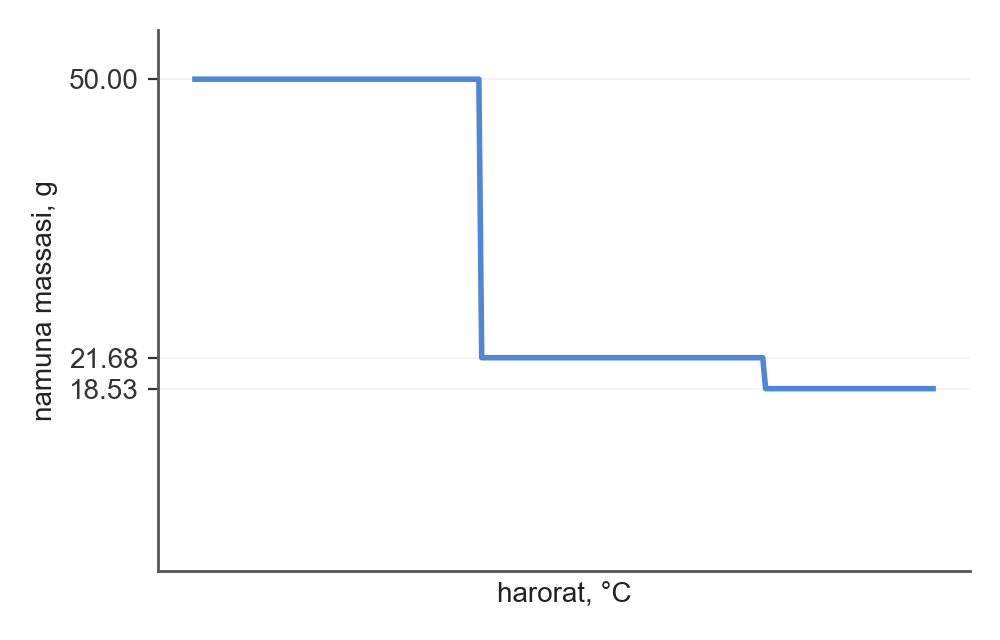
\includegraphics[width=0.86\linewidth]{rasmlar/gen/hy_v16_0.png}\end{center}
To`liq suvsizlangandan keyin qolgan Na\textsubscript{2}CO\textsubscript{3} ning \textbf{massasini (g) toping.}

\noindent A)~\textsl{31,47} \hfill B)~\textsl{21,68} \hfill C)~\textsl{18,53} \hfill D)~\textsl{37,06}\par
\qsep
\noindent\qn{13.} NaCl ning suvli eritmasi inert elektrodlar bilan elektroliz qilinganda qaysi moddalar ajraladi?

\noindent\begin{tabular}{@{}p{0.47\linewidth}@{}p{0.47\linewidth}@{}}
A)~\textsl{Zn, H\textsubscript{2} va O\textsubscript{2}} & B)~\textsl{Ag va O\textsubscript{2}} \\
C)~\textsl{Cu va O\textsubscript{2}} & D)~\textsl{H\textsubscript{2}, Cl\textsubscript{2} va NaOH} \\
\end{tabular}\par
\qsep
\noindent\qn{14.} Rasmdagi o`zgarishlar zanjirida \textit{X} moddaning \textbf{formulasini aniqlang.}
\begin{center}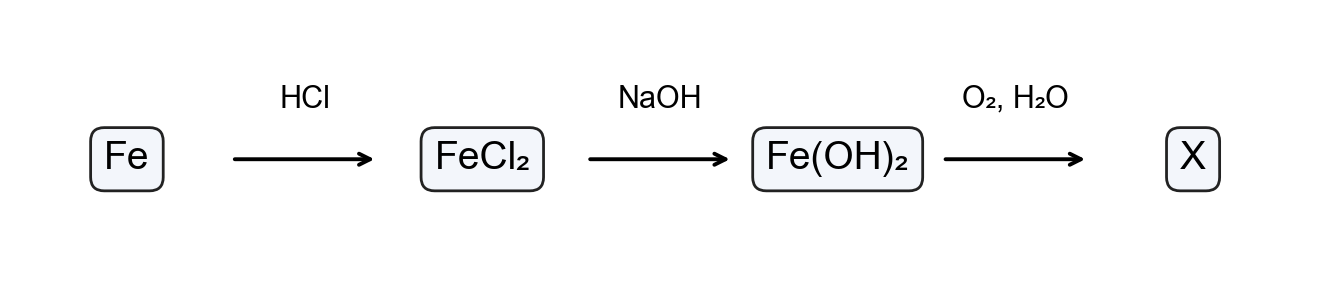
\includegraphics[width=0.86\linewidth]{rasmlar/gen/ci_509279.png}\end{center}

\noindent A)~\textsl{Fe(OH)\textsubscript{3}} \hfill B)~\textsl{FeCl\textsubscript{2}} \hfill C)~\textsl{SO\textsubscript{3}} \hfill D)~\textsl{Fe(OH)\textsubscript{2}}\par
\qsep
\noindent\qn{15.} Cu $\to$ ? $\to$ ? $\to$ ? o`zgarishlar zanjirida (reagentlar: O\textsubscript{2}, H\textsubscript{2}SO\textsubscript{4}, NaOH) 1-bosqichda hosil bo`ladigan modda \textbf{formulasini toping.}

\noindent A)~\textsl{Na\textsubscript{2}SO\textsubscript{3}} \hfill B)~\textsl{Ca(OH)\textsubscript{2}} \hfill C)~\textsl{CuO} \hfill D)~\textsl{NaCl}\par
\qsep
\noindent\qn{16.} NH\textsubscript{3} + H\textsubscript{3}PO\textsubscript{4} $\to$ NH\textsubscript{4}H\textsubscript{2}PO\textsubscript{4} jarayoni uchun 4,48 l (n.sh.) NH\textsubscript{3} olingan (unum 90\%). NH\textsubscript{4}H\textsubscript{2}PO\textsubscript{4} \textbf{miqdorini (mol) aniqlang.}

\noindent A)~\textsl{0,2} \hfill B)~\textsl{0,36} \hfill C)~\textsl{0,18} \hfill D)~\textsl{0,09}\par
\qsep
\noindent\qn{17.} 14,8 g Mg(NO\textsubscript{3})\textsubscript{2} to`liq parchalanguncha qizdirildi. Qattiq qoldiq \textbf{massasini (g) aniqlang.}

\noindent A)~\textsl{4} \hfill B)~\textsl{14,8} \hfill C)~\textsl{8} \hfill D)~\textsl{2}\par
\qsep
\noindent\qn{18.} S + O\textsubscript{2} $\to$ SO\textsubscript{2} jarayoni uchun 8,96 l (n.sh.) O\textsubscript{2} olingan. SO\textsubscript{2} \textbf{hajmini (l, n.sh.) aniqlang.}

\noindent A)~\textsl{17,92} \hfill B)~\textsl{4,48} \hfill C)~\textsl{8,96} \hfill D)~\textsl{13,44}\par
\qsep
\noindent\qn{19.} 2NO + O\textsubscript{2} $\to$ 2NO\textsubscript{2} jarayoni uchun 8,96 l (n.sh.) O\textsubscript{2} olingan. NO \textbf{hajmini (l, n.sh.) aniqlang.}

\noindent A)~\textsl{4,48} \hfill B)~\textsl{17,92} \hfill C)~\textsl{35,84} \hfill D)~\textsl{8,96}\par
\qsep
\noindent\qn{20.} C\textsubscript{3}H\textsubscript{8} + 5O\textsubscript{2} $\to$ 3CO\textsubscript{2} + 4H\textsubscript{2}O jarayoni uchun 8,96 l (n.sh.) C\textsubscript{3}H\textsubscript{8} olingan. CO\textsubscript{2} \textbf{hajmini (l, n.sh.) aniqlang.}

\noindent A)~\textsl{2,99} \hfill B)~\textsl{53,76} \hfill C)~\textsl{26,88} \hfill D)~\textsl{13,44}\par
\qsep
\noindent\qn{21.} 46 g C\textsubscript{2}H\textsubscript{5}OH dan quyidagi ikki bosqichda C\textsubscript{2}H\textsubscript{4}Cl\textsubscript{2} olinadi: 1) C\textsubscript{2}H\textsubscript{5}OH $\to$ C\textsubscript{2}H\textsubscript{4} + H\textsubscript{2}O (unum 80\%); 2) C\textsubscript{2}H\textsubscript{4} + Cl\textsubscript{2} $\to$ C\textsubscript{2}H\textsubscript{4}Cl\textsubscript{2} (unum 75\%). Oxirgi mahsulot C\textsubscript{2}H\textsubscript{4}Cl\textsubscript{2} ning \textbf{massasini (g) toping.}

\noindent A)~\textsl{59,4} \hfill B)~\textsl{74,25} \hfill C)~\textsl{79,2} \hfill D)~\textsl{99}\par
\qsep
\noindent\qn{22.} Arenlar, neft va tabiiy gaz haqida qaysi fikrlar to`g`ri? 1) Neft fraksiyalaridan gazolin 150 \textdegree{}C gacha haydaladi; 2) Benzolda 6 ta sp\textsuperscript{2} gibridlangan uglerod bor; 3) Benzoldan nitrobenzol nitrolash bilan olinadi; 4) Benzol uchun birikish reaksiyalari mutlaqo xos emas

\noindent A)~\textsl{1, 2, 3} \hfill B)~\textsl{1, 4} \hfill C)~\textsl{2, 3} \hfill D)~\textsl{2, 3, 4}\par
\qsep
\noindent\qn{23.} C\textsubscript{2}H\textsubscript{4} + H\textsubscript{2}O (H\textsuperscript{+}) reaksiyasi natijasida qaysi organik modda hosil bo`ladi?

\noindent A)~\textsl{benzol} \hfill B)~\textsl{asetilen} \hfill C)~\textsl{etilen} \hfill D)~\textsl{etanol}\par
\qsep
\noindent\qn{24.} Aldegid va ketonlar haqida qaysi fikrlar to`g`ri? 1) Ketonlar kuchsiz oksidlovchilar bilan oksidlanmaydi; 2) Sirka aldegid Kucherov reaksiyasi bilan olinadi; 3) Aldegidlar "kumush ko`zgu" reaksiyasini beradi; 4) Formaldegid gaz holatda, suvda yaxshi eriydi

\noindent\begin{tabular}{@{}p{0.47\linewidth}@{}p{0.47\linewidth}@{}}
A)~\textsl{1, 2, 4} & B)~\textsl{2, 3, 4} \\
C)~\textsl{1, 3, 4} & D)~\textsl{1, 2, 3, 4} \\
\end{tabular}\par
\qsep
\noindent\qn{25.} C\textsubscript{4}H\textsubscript{8}O\textsubscript{2} karbon kislotalarning izomerlari soni nechta?

\noindent A)~\textsl{3} \hfill B)~\textsl{1} \hfill C)~\textsl{4} \hfill D)~\textsl{2}\par
\qsep
\noindent\qn{26.} 22,2 g propion kislota va 9,2 g etanol dan 80\% unum bilan murakkab efir olindi. Efir \textbf{massasini (g) toping.}

\noindent A)~\textsl{20,4} \hfill B)~\textsl{16,32} \hfill C)~\textsl{24,48} \hfill D)~\textsl{32,64}\par
\qsep
\noindent\qn{27.} 6CO\textsubscript{2} + 6H\textsubscript{2}O $\to$ C\textsubscript{6}H\textsubscript{12}O\textsubscript{6} + 6O\textsubscript{2} reaksiyasida 44 g CO\textsubscript{2} ishtirok etdi. O\textsubscript{2} \textbf{hajmini (l, n.sh.) toping.}

\noindent A)~\textsl{44,8} \hfill B)~\textsl{22,4} \hfill C)~\textsl{11,2} \hfill D)~\textsl{33,6}\par
\qsep
\noindent\qn{28.} Aminlar, aminokislotalar va oqsillar haqida qaysi fikrlar to`g`ri? 1) Nitrobenzoldan anilin Zinin reaksiyasi bilan olinadi; 2) Aminlar kuchsiz asoslar xossasini namoyon qiladi; 3) Aminokislotalar faqat kislotali xossaga ega; 4) Dipeptidda 2 ta peptid bog` bor

\noindent A)~\textsl{4} \hfill B)~\textsl{1, 2} \hfill C)~\textsl{1} \hfill D)~\textsl{3}\par
\qsep
\noindent\qn{29.} Yuqori molekulyar birikmalar haqida qaysi fikrlar to`g`ri? 1) Lavsan poliamid tola; 2) Kapron poliamid tola; 3) Tabiiy kauchuk -- sis-1,4-poliizopren; 4) Teflon --- polivinilxlorid

\noindent A)~\textsl{2, 3} \hfill B)~\textsl{3, 4} \hfill C)~\textsl{1, 2} \hfill D)~\textsl{3}\par
\qsep
\noindent\qn{30.} 100 g 30\% li va 100 g 40\% li NaOH eritmalari aralashtirildi. Yangi eritmaning massa \textbf{ulushini (\%) toping.}

\noindent A)~\textsl{70} \hfill B)~\textsl{35} \hfill C)~\textsl{31,5} \hfill D)~\textsl{38,5}\par
\qsep
\noindent\qn{31.} Kimyo laboratoriyasida ishlash qoidalari haqida qaysi fikrlar to`g`ri? 1) Ishqor teriga tushsa, qo`l suv bilan yuviladi; 2) Probirka qizdirilganda og`zi odamga qaratilmaydi; 3) Zaharli gaz ajraladigan tajriba mo`rili shkafda o`tkaziladi; 4) Konsentrlangan kislotani suvga ohista, aralashtirib quyiladi

\noindent\begin{tabular}{@{}p{0.47\linewidth}@{}p{0.47\linewidth}@{}}
A)~\textsl{1, 2, 3, 4} & B)~\textsl{2, 3, 4} \\
C)~\textsl{1, 3, 4} & D)~\textsl{1, 2, 4} \\
\end{tabular}\par
\qsep
\noindent\qn{32.} Rasmda spirt lampasi alangasi tasvirlangan. Alanganing qaysi qismi eng kam issiq va pilikka yaqin?
\begin{center}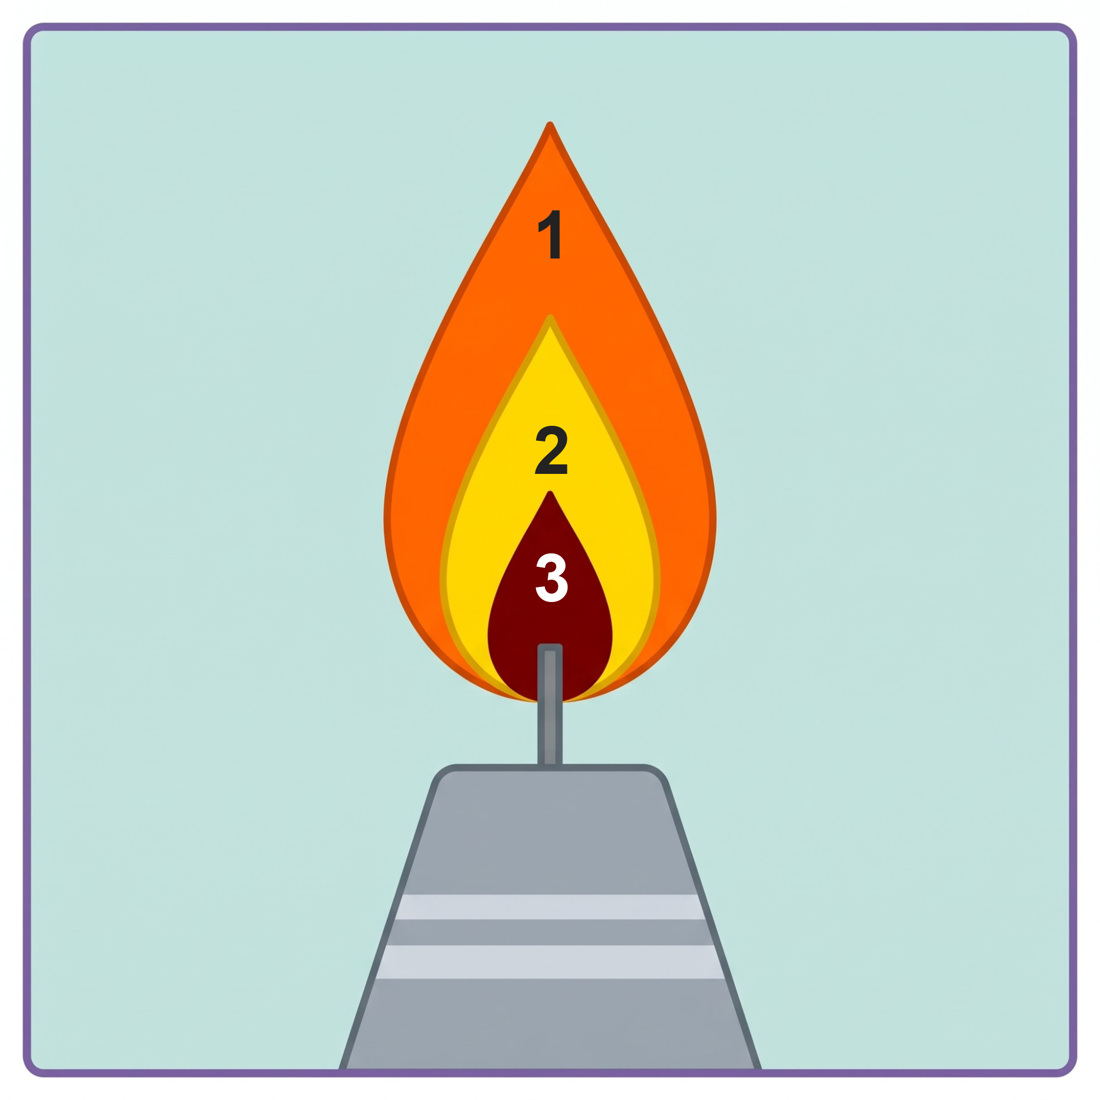
\includegraphics[width=0.86\linewidth]{rasmlar/darslik/d_alanga.png}\end{center}

\noindent\begin{tabular}{@{}p{0.47\linewidth}@{}p{0.47\linewidth}@{}}
A)~\textsl{hamma qismi bir xil} & B)~\textsl{3 -- pastki qism} \\
C)~\textsl{2 -- o`rta qism} & D)~\textsl{1 -- yuqori qism   ---} \\
\end{tabular}\par
\qsep
\end{multicols}
\medskip
\noindent\setlength{\fboxsep}{0pt}\fbox{\begin{tabular}{p{0.74\linewidth}|p{0.2\linewidth}}
\parbox[t]{0.72\linewidth}{\vspace{3pt}\textbf{Topshiriqlar (33--35) va javob variant (A--F)larini o`zaro to`g`ri moslashtiring.} Metan (CH\textsubscript{4}) va propen (C\textsubscript{3}H\textsubscript{6}) dan iborat 7,84 l (n.sh.) aralashma bromli suvdan o`tkazilganda 8 g brom yutildi.
\vspace{3pt}} & \parbox[t]{0.19\linewidth}{\vspace{3pt}A~\textsl{88}\\[3pt]
B~\textsl{11,43}\\[3pt]
C~\textsl{21,43}\\[3pt]
D~\textsl{14,29}\\[3pt]
E~\textsl{1,12}\\[3pt]
F~\textsl{176}}\\ \hline
\parbox[t]{0.72\linewidth}{\vspace{2pt}\textbf{33. Aralashmadagi propen (C\textsubscript{3}H\textsubscript{6}) hajmini (l, n.sh.) aniqlang.}\vspace{2pt}} & \\ \hline
\parbox[t]{0.72\linewidth}{\vspace{2pt}\textbf{34. Aralashmadagi propen (C\textsubscript{3}H\textsubscript{6}) hajmiy ulushini (\%) aniqlang.}\vspace{2pt}} & \\ \hline
\parbox[t]{0.72\linewidth}{\vspace{2pt}\textbf{35. Aralashmani to`liq yoqish uchun zarur havo hajmini (l, n.sh.; havoda 21\% kislorod bor) aniqlang.}\vspace{2pt}} & 
\end{tabular}}
\par\bigskip
\noindent\qn{36.} KMnO\textsubscript{4} + K\textsubscript{2}SO\textsubscript{3} + H\textsubscript{2}O $\to$ MnO\textsubscript{2} + K\textsubscript{2}SO\textsubscript{4} + KOH reaksiya tenglamasini tenglang va barcha koeffitsiyentlar \textbf{yig`indisini aniqlang.}
\javob\qsep
\noindent\qn{37.} 50 g CaCO\textsubscript{3} reaksiyaga kirishdi (CaCO\textsubscript{3} + 2HCl $\to$ CaCl\textsubscript{2} + CO\textsubscript{2} + H\textsubscript{2}O). Ajralgan CO\textsubscript{2} \textbf{hajmini (l, n.sh.) hisoblang.}
\javob\qsep
\noindent\qn{38.} 75,2 g Cu(NO\textsubscript{3})\textsubscript{2} qizdirilganda qisman parchalandi, qattiq qoldiq massasi 53,6 g bo`ldi. Ajralgan gazlar (n.sh.) \textbf{hajmini (l) hisoblang.}
\javob\qsep
\noindent\qn{39.} Etilen va asetilendan iborat 5,6 l (n.sh.) aralashma bromli suvdan o`tkazilganda 56 g brom yutildi. Aralashmadagi asetilenning \textbf{hajmini (l, n.sh.) toping.}
\javob\qsep
\noindent\qn{40.} 14,8 g HCOOC\textsubscript{2}H\textsubscript{5} mo`l NaOH bilan to`liq gidrolizlandi. Hosil bo`lgan spirt \textbf{massasini (g) aniqlang.}
\javob\qsep
\par\bigskip\begin{center}\textbf{\fontsize{13}{15}\selectfont YOZMA ISH}\end{center}
\noindent\qn{41.} \textbf{Topshiriqni bajarish jarayonida barcha reaksiya tenglamalarini yozing. Miqdoriy va arifmetik hisoblashlarni (unga asos bo`lgan usul yoki formulani ko`rsatgan holda) uzviy ketma-ketlikda bajaring.}\par\smallskip
Quyidagi eritmalar berilgan: HCl ning 0,02 mol/l li eritmasi va NaOH ning 0,01 mol/l li eritmasi. Ularni aralashtirib, umumiy hajmi 1 l bo`lgan eritma tayyorlandi (0,3 l HCl eritmasi va 0,7 l NaOH eritmasi). Shuningdek, sirka kislotaning 0,1 mol/l li eritmasida dissotsilanish darajasi 1\%.\par
\noindent 1)Aralashtirilgandan keyingi eritmaning pH ini aniqlang.\par
\noindent 2)Dastlabki HCl eritmasining pH ini hisoblang. 1 l shu eritmadagi HCl massasini (g) ham hisoblang.\par
\noindent 3)Dastlabki NaOH eritmasining pH ini hisoblang.\par
\noindent 4)Sirka kislota eritmasidagi H\textsuperscript{+} ionlari konsentratsiyasini (mol/l) va pH ni aniqlang (lg 2 = 0,3, lg 5 = 0,7 ni ishlating). Shuningdek NaOH eritmasi 100 marta suyultirilsa pH qancha bo`ladi?\par
\noindent 5)Sirka kislotaning dissotsilanish konstantasini hisoblang (K = C$\alpha$\textsuperscript{2}/(1 $-$ $\alpha$)). Shuningdek HCl eritmasi 10 marta suyultirilsa pH necha bo`ladi?\par
\diqqat{Mazkur topshiriq kengaytirilgan javobni talab etib, uning yechilish usuli va shu usul asosidagi barcha hisoblash amallari javoblar varaqasida aks etishi lozim.}\qsep
\noindent\qn{42.} Quyidagi o`zgarishlar zanjirida \textit{X}, \textit{Y}, \textit{Z} noma'lum organik moddalar:\par
\[\setlength{\fboxsep}{0pt}\text{CH\textsubscript{3}Cl}\xrightarrow{\text{Na}}\text{\textit{X}}\xrightarrow{\text{Cl\textsubscript{2}, yorug`lik}}\text{\textit{Y}}\xrightarrow{\text{KOH (suvli)}}\text{\textit{Z}}\xrightarrow{\text{CuO, t\textdegree{}}}\text{CH\textsubscript{3}CHO}\]
\noindent 1)CH\textsubscript{3}Cl $\to$ \textit{X} : reaksiya tenglamasini yozing; hosil bo`lgan moddani nomlang.\par
\noindent 2)\textit{X} $\to$ \textit{Y} : reaksiya tenglamasini yozing; hosil bo`lgan moddani nomlang.\par
\noindent 3)\textit{Y} $\to$ \textit{Z} : reaksiya tenglamasini yozing; hosil bo`lgan moddani nomlang.\par
\noindent 4)\textit{Z} $\to$ CH\textsubscript{3}CHO : reaksiya tenglamasini yozing; hosil bo`lgan moddani nomlang.\par
\diqqat{Mazkur topshiriq kengaytirilgan javobni talab etib, uning yechilish usuli va shu usul asosidagi barcha hisoblash amallari javoblar varaqasida aks etishi lozim.}\qsep
\noindent\qn{43.} \textbf{Topshiriqni bajarish jarayonida barcha reaksiya tenglamalarini yozing. Miqdoriy va arifmetik hisoblashlarni (unga asos bo`lgan usul yoki formulani ko`rsatgan holda) uzviy ketma-ketlikda bajaring.}\par\smallskip
Magniy (Mg) va rux (Zn) dan iborat 15,4 g qotishma mo`l suyultirilgan sulfat kislotada eritildi, bunda 6,72 l (n.sh.) gaz ajraldi. Hosil bo`lgan eritmaga mo`l NaOH eritmasi qo`shildi, hosil bo`lgan cho`kma ajratib olindi va havoda qizdirib quritildi.\par
\noindent 1)Reaksiya tenglamalarini yozing va qotishmadagi har bir metallning massasini (g) aniqlang.\par
\noindent 2)Qotishmadagi Mg ning massa ulushini (\%) hisoblang.\par
\noindent 3)Eritish uchun sarflangan 20\% li H\textsubscript{2}SO\textsubscript{4} eritmasining massasini (g) aniqlang.\par
\noindent 4)Mo`l NaOH qo`shilganda hosil bo`lgan cho`kmaning formulasi va massasini (g) toping (reaksiya tenglamalarini yozing).\par
\noindent 5)Cho`kma havoda to`liq qizdirilganda hosil bo`lgan oksidning massasini (g) hisoblang.\par
\diqqat{Mazkur topshiriq kengaytirilgan javobni talab etib, uning yechilish usuli va shu usul asosidagi barcha hisoblash amallari javoblar varaqasida aks etishi lozim.}\qsep
\newpage
\noindent\textbf{\fontsize{13}{15}\selectfont Nazorat testi}\ \textit{$\cdot$ 16-variant}\hfill \textbf{Javoblar kaliti}\par\smallskip\hrule\smallskip
\textit{Faqat o`qituvchi uchun.}\par\medskip
\noindent\textbf{1--32-savollar}\par\smallskip
\noindent\begin{tabular}{|c|c|c|c|c|c|c|c|c|c|c|c|c|c|c|c|}\hline
\textbf{1} & \textbf{2} & \textbf{3} & \textbf{4} & \textbf{5} & \textbf{6} & \textbf{7} & \textbf{8} & \textbf{9} & \textbf{10} & \textbf{11} & \textbf{12} & \textbf{13} & \textbf{14} & \textbf{15} & \textbf{16}\\\hline
\textsl{B} & \textsl{C} & \textsl{D} & \textsl{D} & \textsl{D} & \textsl{C} & \textsl{A} & \textsl{C} & \textsl{D} & \textsl{B} & \textsl{A} & \textsl{C} & \textsl{D} & \textsl{A} & \textsl{C} & \textsl{C}\\\hline
\textbf{17} & \textbf{18} & \textbf{19} & \textbf{20} & \textbf{21} & \textbf{22} & \textbf{23} & \textbf{24} & \textbf{25} & \textbf{26} & \textbf{27} & \textbf{28} & \textbf{29} & \textbf{30} & \textbf{31} & \textbf{32}\\\hline
\textsl{A} & \textsl{C} & \textsl{B} & \textsl{C} & \textsl{A} & \textsl{A} & \textsl{D} & \textsl{D} & \textsl{D} & \textsl{B} & \textsl{B} & \textsl{B} & \textsl{A} & \textsl{B} & \textsl{A} & \textsl{B}\\\hline
\end{tabular}\par\medskip
\noindent\textbf{33--35-savollar}\par\smallskip
\noindent\begin{tabular}{|c|c|c|}\hline \textbf{No} & \textbf{Javob} & \textbf{Qiymat}\\\hline
33 & \textsl{E} & 1,12\\\hline
34 & \textsl{D} & 14,29\\\hline
35 & \textsl{A} & 88\\\hline
\end{tabular}\par\medskip
\noindent\textbf{36--40-savollar}\par\smallskip
\noindent\begin{tabular}{|c|c|}\hline \textbf{No} & \textbf{To`g`ri javob}\\\hline
36 & 13\\\hline
37 & 11,2\\\hline
38 & 11,2\\\hline
39 & 2,24\\\hline
40 & 9,2\\\hline
\end{tabular}\par\medskip
\noindent\textbf{41--43-topshiriqlar: javoblar}\par\smallskip
\noindent\textbf{41-topshiriq.}\par
\noindent 1) pH = 11\par
\noindent 2) pH = 1,7; 0,73 g\par
\noindent 3) pH = 12\par
\noindent 4) pH = 3; 10\par
\noindent 5) 1,01$\cdot$10\textsuperscript{$-$}5; pH = 2,7\par
\noindent\textbf{42-topshiriq.}\par
\noindent 1) CH\textsubscript{3}Cl + Na $\to$ C\textsubscript{2}H\textsubscript{6} (etan)\par
\noindent 2) C\textsubscript{2}H\textsubscript{6} + Cl\textsubscript{2}, yorug`lik $\to$ C\textsubscript{2}H\textsubscript{5}Cl (xloretan)\par
\noindent 3) C\textsubscript{2}H\textsubscript{5}Cl + KOH (suvli) $\to$ C\textsubscript{2}H\textsubscript{5}OH (etanol)\par
\noindent 4) C\textsubscript{2}H\textsubscript{5}OH + CuO, t\textdegree{} $\to$ CH\textsubscript{3}CHO (sirka aldegid (etanal))\par
\noindent\textbf{43-topshiriq.}\par
\noindent 1) 2,4 g; 13 g\par
\noindent 2) 15,6\%\par
\noindent 3) 147 g\par
\noindent 4) 5,8 g\par
\noindent 5) 4 g\par
\par\bigskip\noindent\textbf{Mavzular taqsimoti}\par\smallskip
{\small\noindent\begin{longtable}{|c|p{7.2cm}|p{5.4cm}|c|}\hline \textbf{No} & \textbf{Mavzu} & \textbf{Tekshiriladigan ko`nikma} & \textbf{Ball}\\\hline
1 & Tirkashev VI bob (muvozanat, jadval) & Jadval tahlili & 1\\\hline
2 & 11-sinf (Mendeleyev--Klapeyron) & Hisoblash va masala yechish & 1\\\hline
3 & 8-sinf; Tirkashev II bob (kimyoviy bog`lanish) & Bilim va tushunish & 1\\\hline
4 & Tirkashev VI bob (tezlik, jadval) & Jadval tahlili & 1\\\hline
5 & Tirkashev \textit{V} bob; 11-sinf 7-bob & Bilim va tushunish & 1\\\hline
6 & 7-sinf (Avogadro) & Hisoblash va masala yechish & 1\\\hline
7 & 8-sinf; Tirkashev VI bob & Hisoblash va masala yechish & 1\\\hline
8 & 11-sinf 4-bob (normal konsentratsiya) & Hisoblash va masala yechish & 1\\\hline
9 & Tirkashev \textit{V} bob; Tashev (HNO\textsubscript{3}, H\textsubscript{2}SO\textsubscript{4}) & Hisoblash va masala yechish & 1\\\hline
10 & Tirkashev VI bob (kimyoviy muvozanat) & Hisoblash va masala yechish & 1\\\hline
11 & 9-sinf (gidroliz); Tirkashev IV bob & Bilim va tushunish & 1\\\hline
12 & 7-sinf (kristallogidratlar) & Grafik tahlili & 1\\\hline
13 & 11-sinf 8-bob; Tirkashev \textit{V} bob (elektroliz) & Bilim va tushunish & 1\\\hline
14 & 9-sinf (genetik bog`lanish) & Rasm bo`yicha tahlil & 1\\\hline
15 & 8-sinf; 9-sinf (genetik bog`lanish) & Bilim va tushunish & 1\\\hline
16 & 9-sinf; Tirkashev (mineral o`g`itlar/nodir gazlar, hisob) & Hisoblash va masala yechish & 1\\\hline
17 & Tashev (nitratlar termik parchalanishi) & Hisoblash va masala yechish & 1\\\hline
18 & 9-sinf; Tirkashev (S/SO\textsubscript{2}/H\textsubscript{2}SO\textsubscript{4}, hisob) & Hisoblash va masala yechish & 1\\\hline
19 & 9-sinf; Tirkashev (N/NH\textsubscript{3}/HNO\textsubscript{3}, hisob) & Hisoblash va masala yechish & 1\\\hline
20 & 10-sinf (alkan, hisob) & Hisoblash va masala yechish & 1\\\hline
21 & 10-sinf (ikki bosqichli hisob) & Hisoblash va masala yechish & 1\\\hline
22 & 10-sinf (mavzuga oid paragraflar); Abdusamatov & Bilim va tushunish & 1\\\hline
23 & 10-sinf (olinish usullari) & Bilim va tushunish & 1\\\hline
24 & 10-sinf (mavzuga oid paragraflar); Abdusamatov & Bilim va tushunish & 1\\\hline
25 & 10-sinf \S{}6, \S{}12, \S{}20, \S{}28 (izomeriya) & Bilim va tushunish & 1\\\hline
26 & 10-sinf \S{}28 (efirlanish) & Hisoblash va masala yechish & 1\\\hline
27 & 10-sinf (ugl, hisob) & Hisoblash va masala yechish & 1\\\hline
28 & 10-sinf (mavzuga oid paragraflar); Abdusamatov & Bilim va tushunish & 1\\\hline
29 & 10-sinf (mavzuga oid paragraflar); Abdusamatov & Bilim va tushunish & 1\\\hline
30 & Tirkashev III bob (eritmalar) & Hisoblash va masala yechish & 1\\\hline
31 & 7-sinf (xavfsizlik qoidalari); 10-sinf lab. & Bilim va tushunish & 1\\\hline
32 & 7-sinf (5-rasm) & Rasm bo`yicha tahlil & 1\\\hline
33--35 & Aralash masala (moslashtirish) & Ko`p bosqichli hisob & 3\\\hline
36--40 & Qisqa javobli masalalar & Hisoblash & 5\\\hline
41--43 & Yozma ish & Usul va hisob (M, A) & 75\\\hline
\end{longtable}}
\end{document}
